\subsection{Quantum Fourier Transform}
To lower down the complexity of order-finding we will utilize a variant of Fourier Transform over the group $\mathbb{Z}_N$, where $N=0^n$, which is a unitary operation over $\complex^{2^n}$. We present a way to implement it using $O(n^2)$ quantum gates which is exponentially faster than a classical approach, using FFT would take $O(n2^n)$ \cite{cormen2009}. However classical FFT outputs a vector from which we can read the result in its entirety, whereas QFT outputs an entangled quantum register that represents the same result, but upon measurement some information is lost. We cannot retrieve the full result, which means that QFT is only viable for certain applications. Luckily, one of them is order-finding.
\\\\
The Quantum Fourier Transform is formally defined by the operation acting on a qubit belonging to the quantum register of length $n$, as
\begin{align*}
    QFT(\ket{x})=\frac{1}{\sqrt{N}}\sum_{y=1}^{N} e^{2\pi i xy/N}\ket{y}
\end{align*}
We will compute it sequentially for each qubit, for $i$-th qubit we first apply a Hadamard gate on it to allow quantum interference, next we apply $n-i$ controlled phase gates to qubit $i$ taking qubits $\{i+1, n\}$ as control. Controlled phase gates take two qubits, target and control and apply a phase shift $e^{\pi / 2^k}$ to the target qubit if the control qubit is in state $\ket{1}$, where $k$ denotes the distance between qubits, we attach a visualization of the quantum circuit for $3$ qubit system \ref{fig:qft}.
\begin{figure}[ht!]
    \centering
    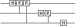
\includegraphics[width=0.7\linewidth]{figures/qft.pdf}
    \caption{QFT diagram for an example, 3 qubit system}
    \label{fig:qft}
\end{figure}
